\documentclass[titlepage, a4paper]{article}
\usepackage[english]{babel}
\usepackage[utf8]{inputenc}
\usepackage{graphicx}
\usepackage{color}
\usepackage{mathtools}
\usepackage{float}
\usepackage[parfill]{parskip}
\usepackage[margin=10pt,font=small,labelfont=bf,labelsep=endash]{caption}
\usepackage{epstopdf}
\usepackage{listings}
\epstopdfsetup{suffix=}
\DeclareGraphicsExtensions{.ps}
\DeclareGraphicsRule{.ps}{pdf}{.pdf}{`ps2pdf -dEPSCrop -dNOSAFER #1 \noexpand\OutputFile}

\lstset{literate=%
    {å}{{\r{a}}}1
    {ä}{{\"a}}1
    {ö}{{\"o}}1
    {Å}{{\r{A}}}1
    {Ä}{{\"A}}1
    {Ö}{{\"O}}1
}

\newcommand{\todo}[1] {\textbf{\textcolor{red}{#1}}}

\usepackage{fancyhdr}
\fancyhead[L]{}
\pagestyle{fancy}
\rhead{Alexander Yngve \\ Pål Kastman}
\chead{TDDC78}
\thispagestyle{empty}

\begin{document}

{\ }\vspace{45mm}

\begin{center}
  \Huge \textbf{TDDC78: Lab Report}
\end{center}
\begin{center}
  \Large Lab 5: Particle Simulation with MPI
\end{center}

\vspace{250pt}

\begin{center}
  \begin{tabular}{|*{3}{p{40mm}|}}
    \hline
    \textbf{Name} & \textbf{PIN} & \textbf{Email} \\ \hline
           {Alexander Yngve} & {930320-6651} & {aleyn573@student.liu.se} \\ \hline
           {Pål Kastman} & {851212-7575} & {palka285@student.liu.se} \\ \hline
  \end{tabular}
\end{center}
\newpage

\tableofcontents
\thispagestyle{empty}
\newpage

\section{Introduction}
In this lab we were to do a particle simulation and verify the gas law $pV=nRT$ using the MPI framework.

\section{Our implementation}
We split the area in regions along the vertical axis, just as in the first lab. We then iterate over the amount of time.

In each time step the following is performed:

\begin{enumerate}
\item {
  For all particles:
  \begin{enumerate}
  \item The particle is checked for collisions.
  \item If a collision occurs, the affected particles are moved in new directions. Otherwise the particle is moved in its current trajectory.
  \item The particle is checked if it should be transferred up or down to another process.
  \item The particle is checked for collisions against the walls. If there is a wall collision the particles momentum is added to the processes local momentum and the particle is moved.
  \end{enumerate}
}
\item Particles are sent upwards.
\item Particles are recieved from below.
\item Particles are sent downwards.
\item Particles are recieved from above.
\end{enumerate}

The total momentum is then accumulated with MPI\_Reduce and thereafter the pressure can be calculated.

\section{Results}
The results can be seen in table \ref{tab:results} and figure \ref{fig:exe_times}.

\begin{table}[H]
  \centering
  \caption{Results from exectuions on Triolith.}
  \begin{tabular}{|*{3}{p{20mm}|}}
    \hline
    \textbf{Cores} & \textbf{Pressure} & \textbf{Time} \\ \hline
           {1} & {1.7690} & {5.8408} \\ \hline
           {2} & {1.5407} & {2.0158} \\ \hline
           {4} & {1.3983} & {0.9994} \\ \hline
           {8} & {1.2400} & {0.7063} \\ \hline
           {16} & {1.1500} & {0.5550} \\ \hline
  \end{tabular}
  \label{tab:results}
\end{table}

\begin{figure}[H]
  \centering
  \scalebox{0.48}{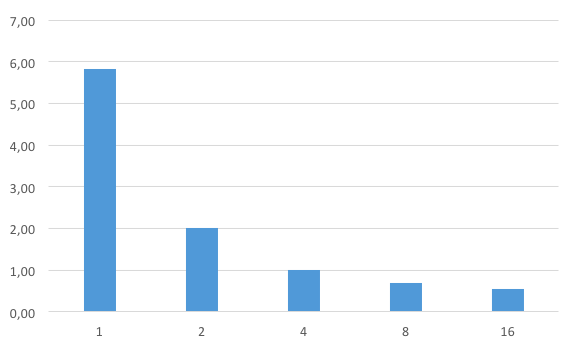
\includegraphics{img/exe_times.png}}
  \caption{Execution times for different number of cores.}
  \label{fig:exe_times}
\end{figure}

\section{Discussion}
As can be seen in table \ref{tab:results} the pressure changes with the amount of cores. This is of course not correct. This is due to the way the parallelisation is implemented. If two particles collide across a border between two processes, the collsion wont be detected. They will just pass through eachother and be transferred to the other process. With an increasing number of cores, there will be more borders that this can happen on, which makes the pressure deviate more from the correct value (which is the value obtained using one core).

\end{document}
